\chapter{Практическая часть}


\section{Внедрение API Gateway в архитектуру информационно-аналитической системы}

\subsection{Анализ требований и постановка исследовательских задач}

Разработка архитектурного решения для информационно-аналитического ресурса «Православный ландшафт таежной Сибири» инициируется комплексным анализом функциональных и нефункциональных требований к распределенной системе обработки исторических данных. Фундаментальным требованием выступает обеспечение высокодоступного и отказоустойчивого доступа к гетерогенным массивам исторической информации, что обусловливает необходимость применения современных архитектурных паттернов и технологических решений.

Требование масштабируемости определяется экспоненциальным ростом объемов обрабатываемых данных и интенсивности пользовательских запросов, что предполагает реализацию механизмов горизонтального масштабирования и динамического распределения вычислительной нагрузки. Особую значимость приобретает обеспечение информационной безопасности и защиты персональных данных в контексте обработки исторических документов, содержащих конфиденциальную информацию о религиозных объектах и персоналиях. Гибкость маршрутизации и обработки разнородных запросов представляет собой критически важное требование, обусловленное полиморфной природой аналитических задач и множественностью клиентских интерфейсов.

\subsection{Компонентная декомпозиция архитектурного решения}

Архитектурная организация системы базируется на принципах микросервисной декомпозиции с выделением следующих фундаментальных компонентов. Spring Cloud Gateway выступает в качестве центрального координирующего элемента, реализующего функции интеллектуальной маршрутизации запросов и применения комплексных политик безопасности. Данный компонент обеспечивает абстрагирование внутренней топологии микросервисной экосистемы от внешних потребителей, реализуя принцип инкапсуляции на архитектурном уровне.

Микросервисная инфраструктура представлена специализированными вычислительными модулями, каждый из которых инкапсулирует определенную область предметной логики. Сервисы обработки исторических данных реализуют алгоритмы семантического анализа и контекстуальной интерпретации архивных документов. Подсистема управления пользовательскими контекстами обеспечивает персонализацию аналитических процессов и поддержку многопользовательских сценариев работы. Модули генерации отчетов применяют методы визуальной аналитики для представления результатов исследований в различных форматах.

Персистентный уровень архитектуры реализован через гибридную модель хранения, сочетающую реляционные системы управления базами данных для структурированной информации о православных объектах культурного наследия и документо-ориентированные хранилища для неструктурированных исторических материалов. Применение полиглотной персистентности позволяет оптимизировать характеристики производительности для различных типов аналитических запросов. Интерфейсный уровень представлен совокупностью веб-приложений, обеспечивающих многоканальный доступ к функциональности системы с учетом специфики различных категорий пользователей.


\section{Архитектурная организация микросервисной системы аналитики исторических данных}

\subsection{Компонентная структура информационно-аналитического ресурса}

Архитектура современных информационно-аналитических систем требует комплексного подхода к организации вычислительных ресурсов и обработке данных. В рамках разработки онлайн-ресурса «Православный ландшафт таежной Сибири» была спроектирована микросервисная архитектура, обеспечивающая модульность, масштабируемость и отказоустойчивость системы. Каждый микросервис в данной архитектуре представляет собой автономную функциональную единицу, ответственную за конкретную область предметной логики: обработку исторических данных, управление пользовательскими сессиями, генерацию аналитических отчетов и визуализацию геопространственной информации.

Персистентный слой системы реализован посредством гибридного подхода к хранению данных, сочетающего реляционные и документо-ориентированные базы данных для оптимального представления структурированной информации о православных объектах культурного наследия и неструктурированных исторических документов. Интерфейсный уровень представлен веб-приложениями, обеспечивающими многоканальный доступ к функциональности системы.

\subsection{Проблематика архитектуры прямого обращения к микросервисам}

До внедрения централизованного API-шлюза архитектура системы базировалась на принципе прямой маршрутизации запросов к отдельным микросервисам. Данный подход демонстрировал ряд существенных ограничений, препятствующих эффективному функционированию распределенной системы.

Первичной проблемой являлось обеспечение информационной безопасности. Прямой доступ к микросервисам экспоненциально увеличивал поверхность атаки системы, создавая множественные векторы потенциальных угроз. Отсутствие единой точки контроля делало практически невозможным применение консистентных политик безопасности и мониторинга аномальной активности в режиме реального времени. Каждый микросервис требовал индивидуальной реализации механизмов аутентификации и авторизации, что приводило к дублированию кода и повышало вероятность возникновения уязвимостей.

Версионирование API представляло собой отдельную категорию сложностей. Наличие множественных эндпоинтов у каждого микросервиса, включая различные версии интерфейсов в рамках одного сервиса, создавало проблему управления жизненным циклом API. Клиентские приложения вынуждены были поддерживать сложную логику маршрутизации и обработки различных версий интерфейсов, что существенно усложняло процесс разработки и поддержки.

Дополнительно следует отметить проблему кросс-функциональных требований (cross-cutting concerns), таких как логирование, мониторинг производительности и обработка ошибок, которые требовали реализации в каждом микросервисе отдельно. Это приводило к нарушению принципа DRY (Don't Repeat Yourself) и усложняло поддержку единообразия системы.
Архитектурная схема работы проекта до внедрения выглядела сле-
дующим образом~\ref{fig:wo-gateway-project}.

\begin{figure}[htbp]
    \centering
    % Placeholder для диаграммы деятельности OpenID
    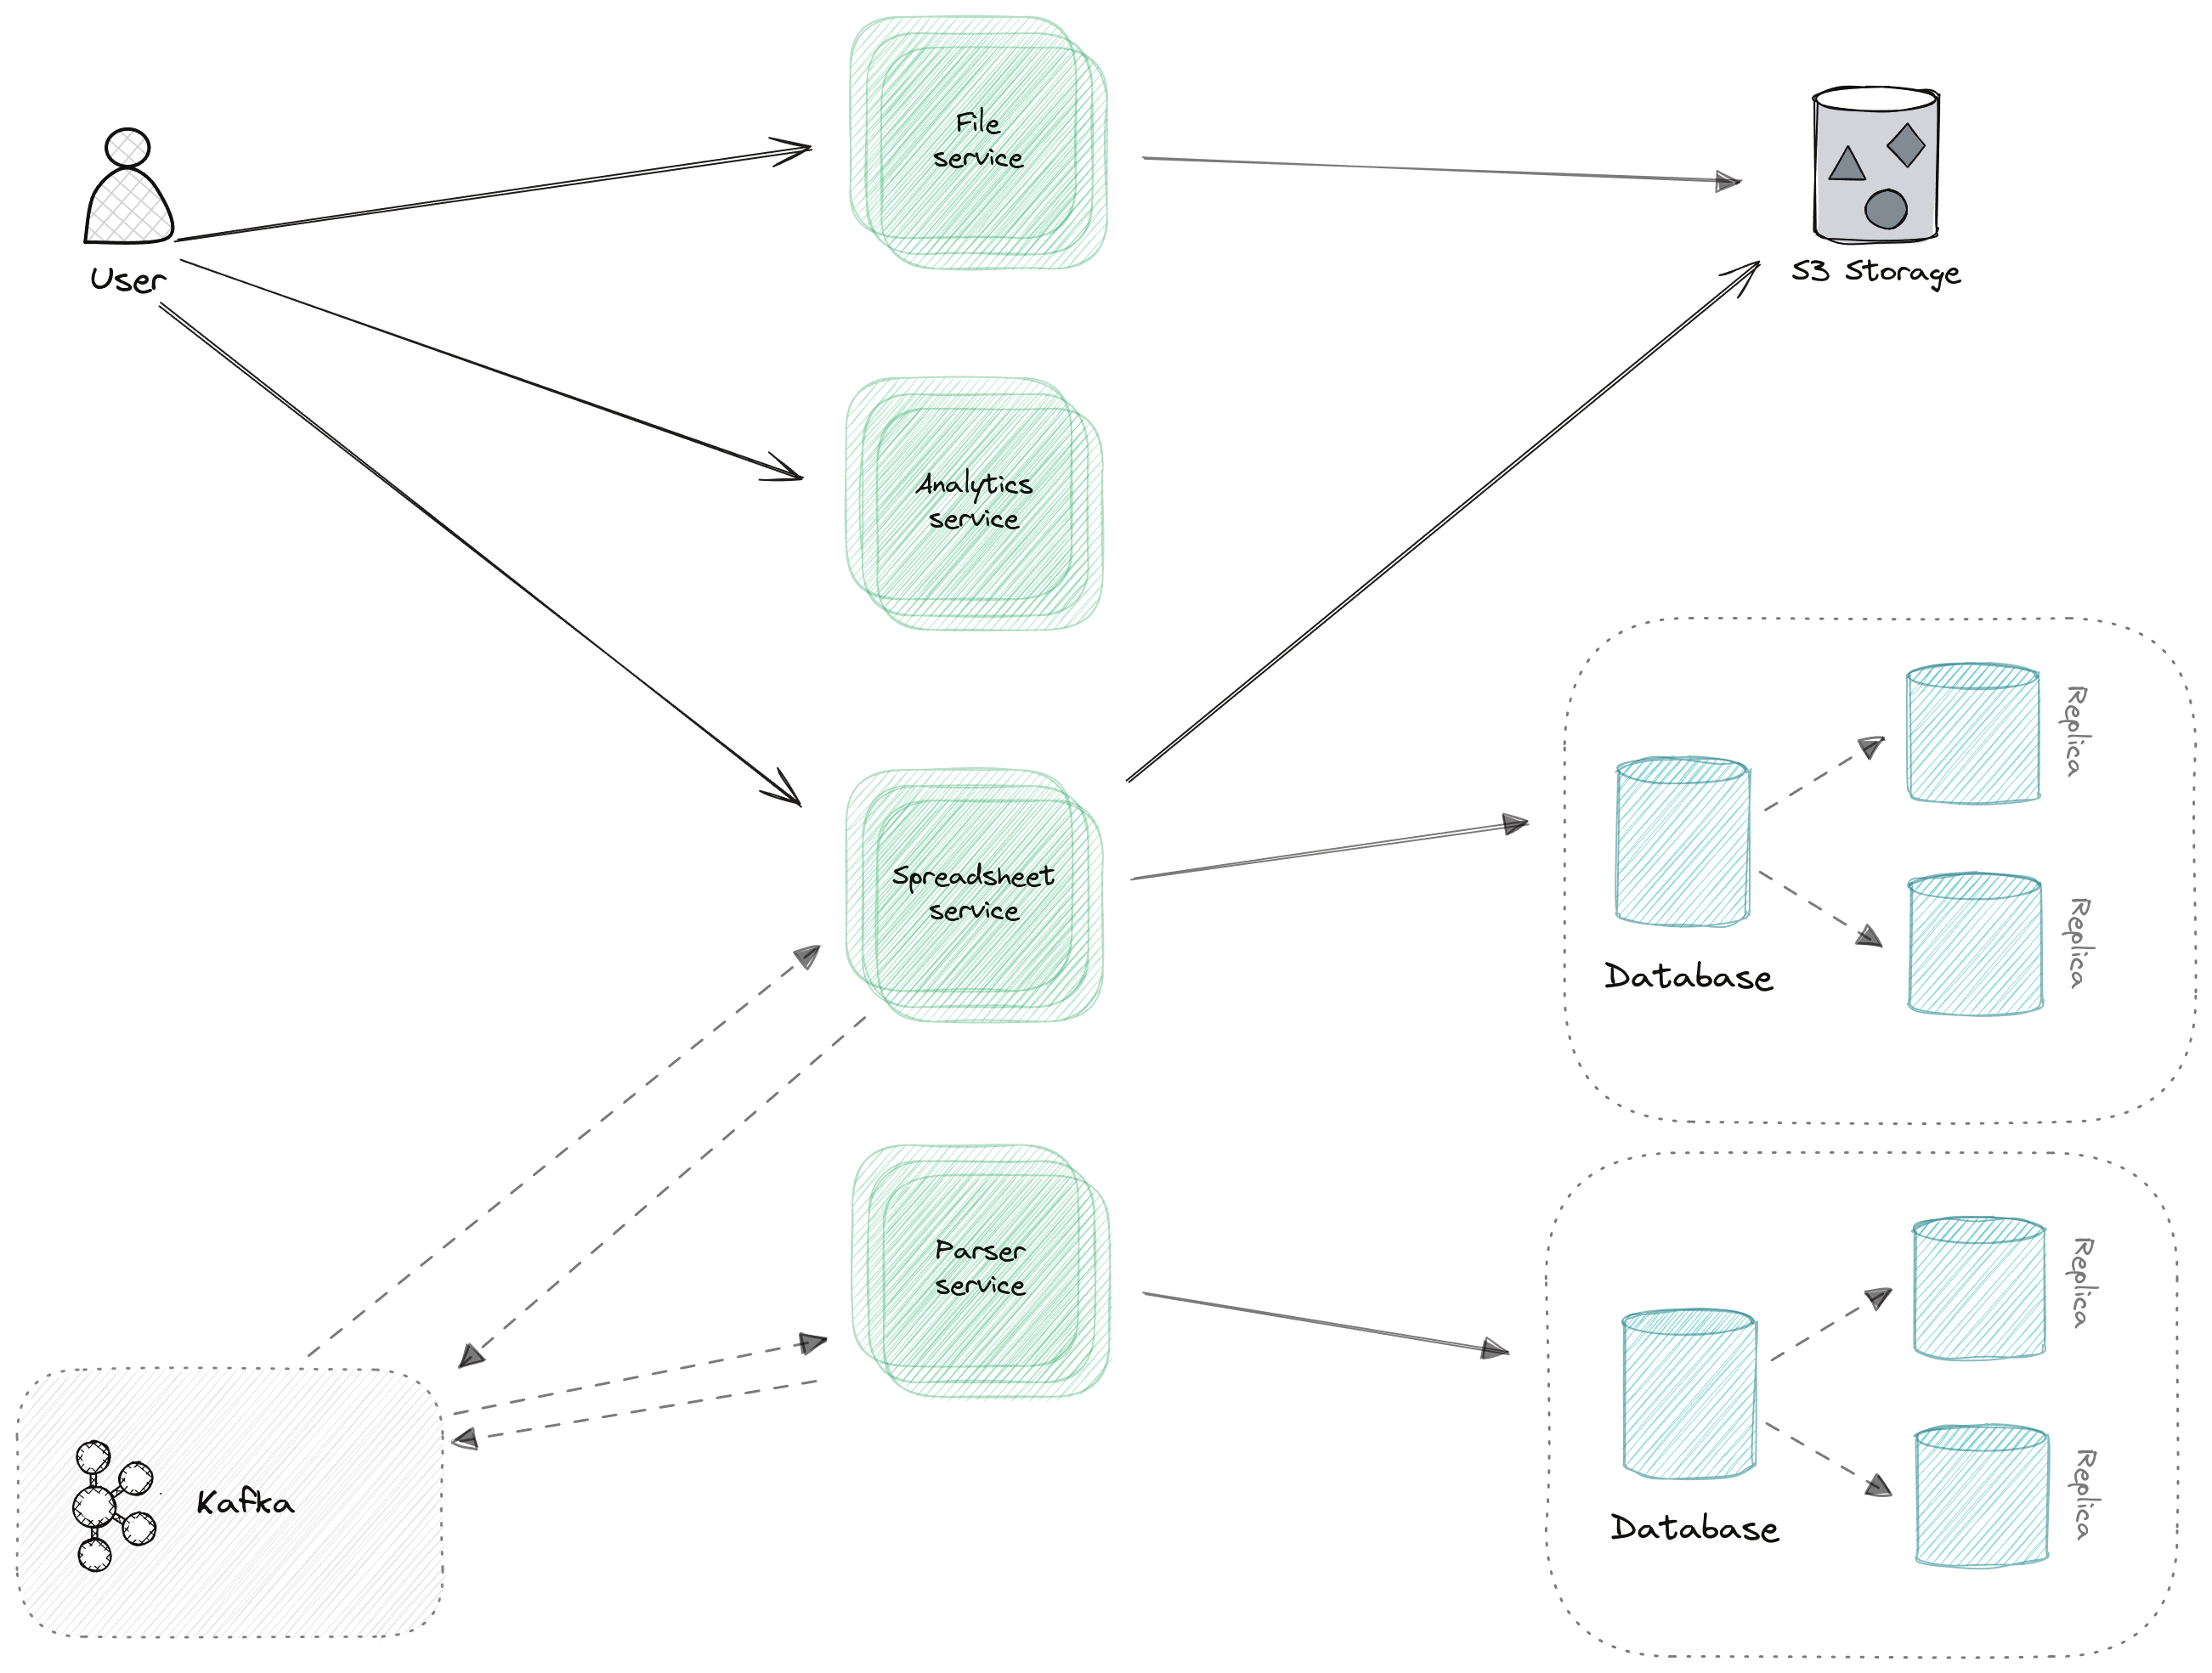
\includegraphics[width=0.7\textwidth]{Dissertation/images/wo-gateway-project}
    \caption{Архитектура без фильтра}
    \label{fig:wo-gateway-project}
\end{figure}

\subsection{Концептуальное проектирование архитектуры с применением Spring Cloud Gateway}

Для решения обозначенных проблем была разработана архитектурная концепция, основанная на паттерне API Gateway с использованием Spring Cloud Gateway в качестве технологической платформы. Данное решение обеспечивает создание единой точки входа для всех клиентских запросов, реализуя принцип инкапсуляции внутренней структуры микросервисной системы.

Спроектированная архитектура базируется на реактивной модели обработки запросов, что обеспечивает высокую производительность при минимальном потреблении системных ресурсов. Spring Cloud Gateway, построенный на основе Project Reactor и Spring WebFlux, позволяет эффективно обрабатывать большое количество конкурентных соединений, используя неблокирующий ввод-вывод.

Была спроектирована схема, которая представлена на рисунке~\ref{fig:w-gateway-project}.
\begin{figure}[htbp]
    \centering
    % Placeholder для диаграммы деятельности OpenID
    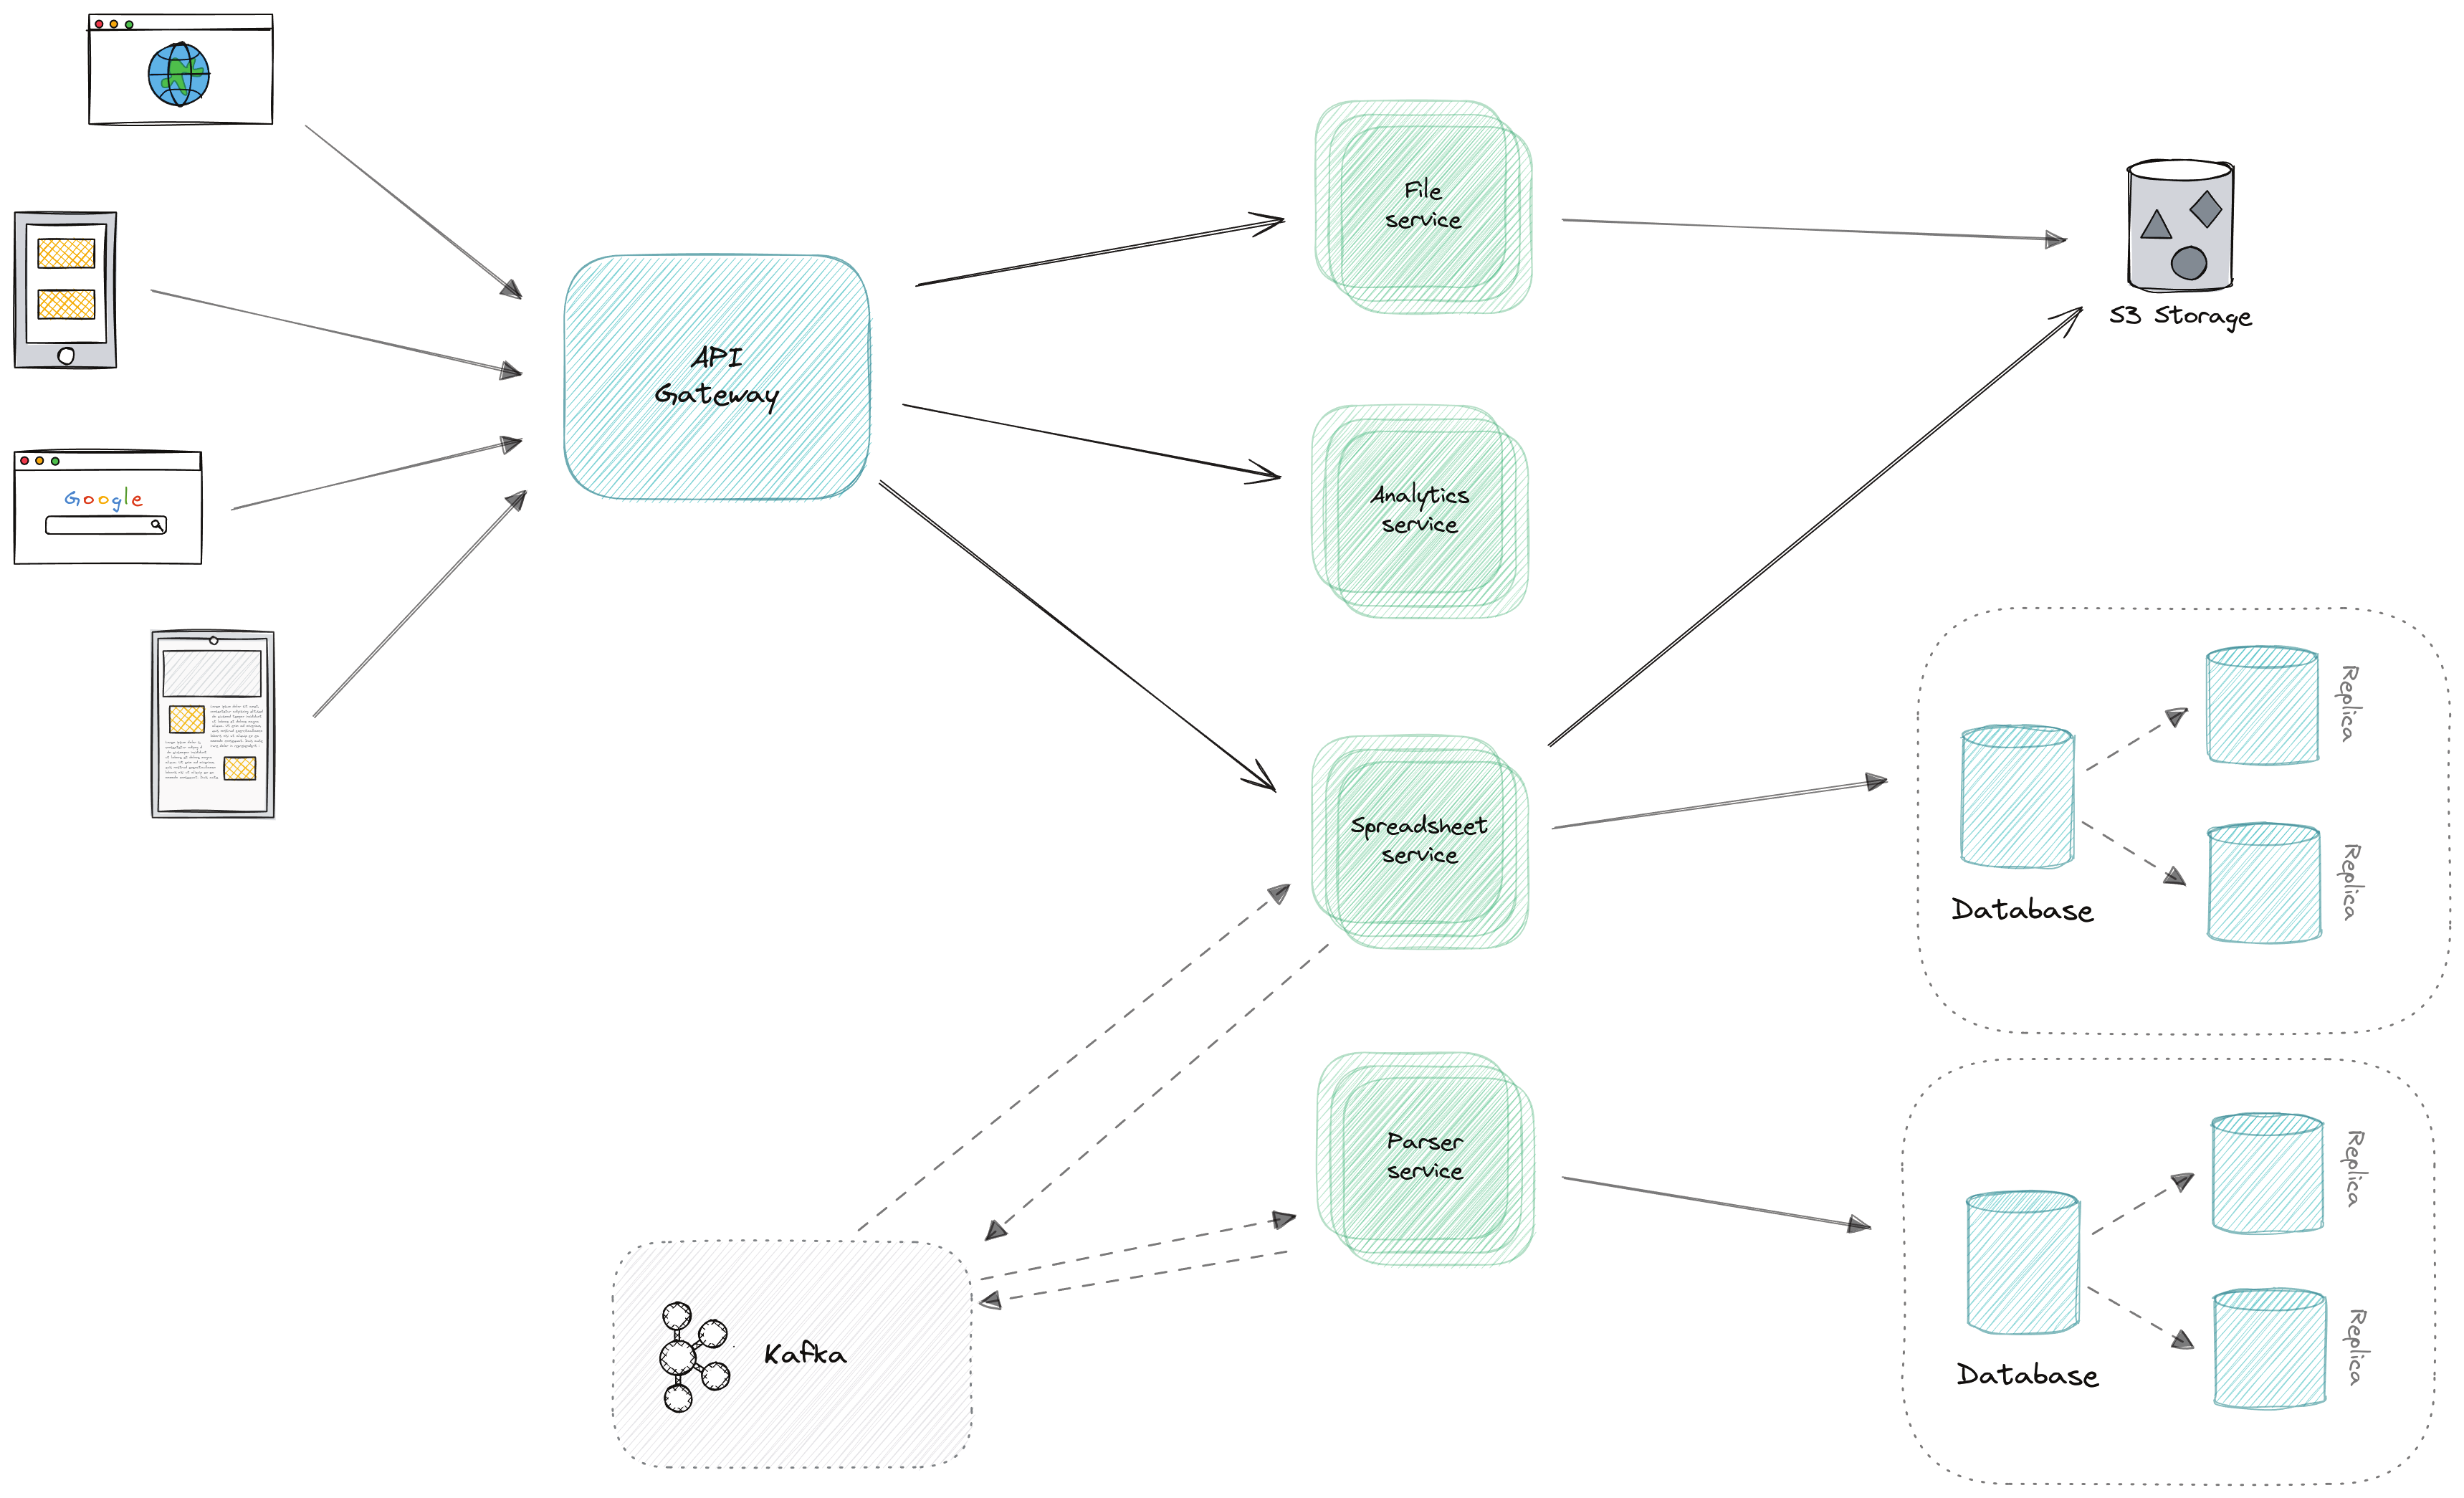
\includegraphics[width=0.7\textwidth]{Dissertation/images/w_gw_proj}
    \caption{Архитектура с фильтра}
    \label{fig:w-gateway-project}
\end{figure}

\subsection{Реализация механизмов балансировки нагрузки и маршрутизации}

Ключевым компонентом реализованной архитектуры является конфигурация балансировщика нагрузки, интегрированного в Spring Cloud Gateway. Был имплементирован алгоритм кругового перебора (Round Robin), обеспечивающий равномерное распределение входящих запросов между доступными экземплярами микросервисов. Данный подход позволяет достичь оптимального использования вычислительных ресурсов и повысить отказоустойчивость системы.

Конфигурация балансировщика нагрузки представлена в следующем примере:

\begin{lstlisting}
spring:
  cloud:
    gateway:
      routes:
        - id: user-service
          uri: lb://user-service
          predicates:
            - Path=/api/users/**
          filters:
            - name: CircuitBreaker
              args:
                name: user-service-cb
                fallbackUri: forward:/fallback/users
    loadbalancer:
      ribbon:
        enabled: false
      configurations: default
      health-check:
        enabled: true
        interval: 30s
\end{lstlisting}

Механизм маршрутизации реализован через декларативную конфигурацию, определяющую правила перенаправления запросов на основе анализа путей и применения цепочек фильтров. Фильтры обеспечивают трансформацию запросов и ответов, включая модификацию заголовков, перезапись путей и добавление метаинформации для трассировки распределенных транзакций.

Пример конфигурации маршрутизации с применением фильтров:

\begin{lstlisting}
@Configuration
public class GatewayConfig {

    @Bean
    public RouteLocator customRouteLocator(RouteLocatorBuilder builder) {
        return builder.routes()
            .route("user-service", r -> r
                .path("/api/users/**")
                .filters(f -> f
                    .addRequestHeader("X-Gateway-Version", "1.0")
                    .addResponseHeader("X-Response-Time",
                        String.valueOf(System.currentTimeMillis()))
                    .rewritePath("/api/users/(?<segment>.*)",
                        "/users/${segment}")
                    .circuitBreaker(c -> c
                        .name("user-service-cb")
                        .fallbackUri("forward:/fallback/users")))
                .uri("lb://user-service"))
            .route("order-service", r -> r
                .path("/api/orders/**")
                .and()
                .method("GET", "POST")
                .filters(f -> f
                    .stripPrefix(1)
                    .addRequestParameter("source", "gateway")
                    .retry(retryConfig -> retryConfig
                        .retries(3)
                        .backoff(Duration.ofSeconds(1),
                               Duration.ofSeconds(10), 2, true)))
                .uri("lb://order-service"))
            .build();
    }
}
\end{lstlisting}

Дополнительно был реализован кастомный фильтр для логирования и мониторинга запросов:

\begin{lstlisting}
@Component
public class RequestLoggingFilter implements GlobalFilter, Ordered {

    private static final Logger logger =
        LoggerFactory.getLogger(RequestLoggingFilter.class);

    @Override
    public Mono<Void> filter(ServerWebExchange exchange,
                           GatewayFilterChain chain) {
        ServerHttpRequest request = exchange.getRequest();
        String traceId = UUID.randomUUID().toString();

        // Добавление заголовка трассировки
        ServerHttpRequest mutatedRequest = request.mutate()
            .header("X-Trace-ID", traceId)
            .build();

        ServerWebExchange mutatedExchange =
            exchange.mutate().request(mutatedRequest).build();

        logger.info("Incoming request: {} {} - Trace ID: {}",
                   request.getMethod(),
                   request.getURI(),
                   traceId);

        return chain.filter(mutatedExchange)
            .doOnSuccess(aVoid -> logger.info(
                "Request completed successfully - Trace ID: {}", traceId))
            .doOnError(throwable -> logger.error(
                "Request failed - Trace ID: {} - Error: {}",
                traceId, throwable.getMessage()));
    }

    @Override
    public int getOrder() {
        return -1; // Высокий приоритет выполнения
    }
}
\end{lstlisting}

\subsection{Обеспечение транспортной безопасности через SSL/TLS}

Критически важным аспектом архитектуры является обеспечение конфиденциальности и целостности передаваемых данных. Реализация SSL/TLS шифрования на уровне API Gateway обеспечивает защиту всех коммуникаций между клиентскими приложениями и микросервисной инфраструктурой.

{В контексте российской цифровой инфраструктуры особую актуальность приобретает возможность использования отечественных сертификатов безопасности, предоставляемых через портал Госуслуг}. Министерство цифрового развития предоставляет возможность получения стандартных OV (Organization Validation) и базовых DV (Domain Validation) сертификатов, что обеспечивает независимость от иностранных центров сертификации.

Процесс интеграции SSL включает генерацию криптографических ключей, конфигурацию хранилища ключей в формате PKCS12 и настройку Spring Boot для использования защищенных соединений. Все клиентские приложения требуют соответствующей модификации для перехода на HTTPS-протокол, что обеспечивает сквозное шифрование на всех уровнях взаимодействия.


\section{Централизованное управление конфигурацией в микросервисной архитектуре}

\subsection{Архитектурные принципы сервера конфигурации}

Проектирование централизованного сервера конфигурации представляет собой фундаментальный аспект построения управляемой микросервисной экосистемы. Данный подход обеспечивает единообразное управление конфигурационными параметрами, гарантирует их консистентность и обеспечивает возможность динамического обновления без перезапуска приложений. Централизация конфигурационного управления существенно снижает операционную сложность администрирования распределенных систем и минимизирует риски, связанные с рассинхронизацией конфигураций между средами развертывания.

Архитектура сервера конфигурации базируется на принципе разделения конфигурационных профилей для различных сред выполнения, что позволяет поддерживать изолированные настройки для среды разработки, тестирования и продуктивной эксплуатации. Данный подход обеспечивает безопасное продвижение изменений через различные стадии жизненного цикла приложения.

В ходе работы была спроектированная схема, представленная на рисунке~\ref{fig:cfg_prj}.

\begin{figure}[htbp]
    \centering
    % Placeholder для диаграммы деятельности OpenID
    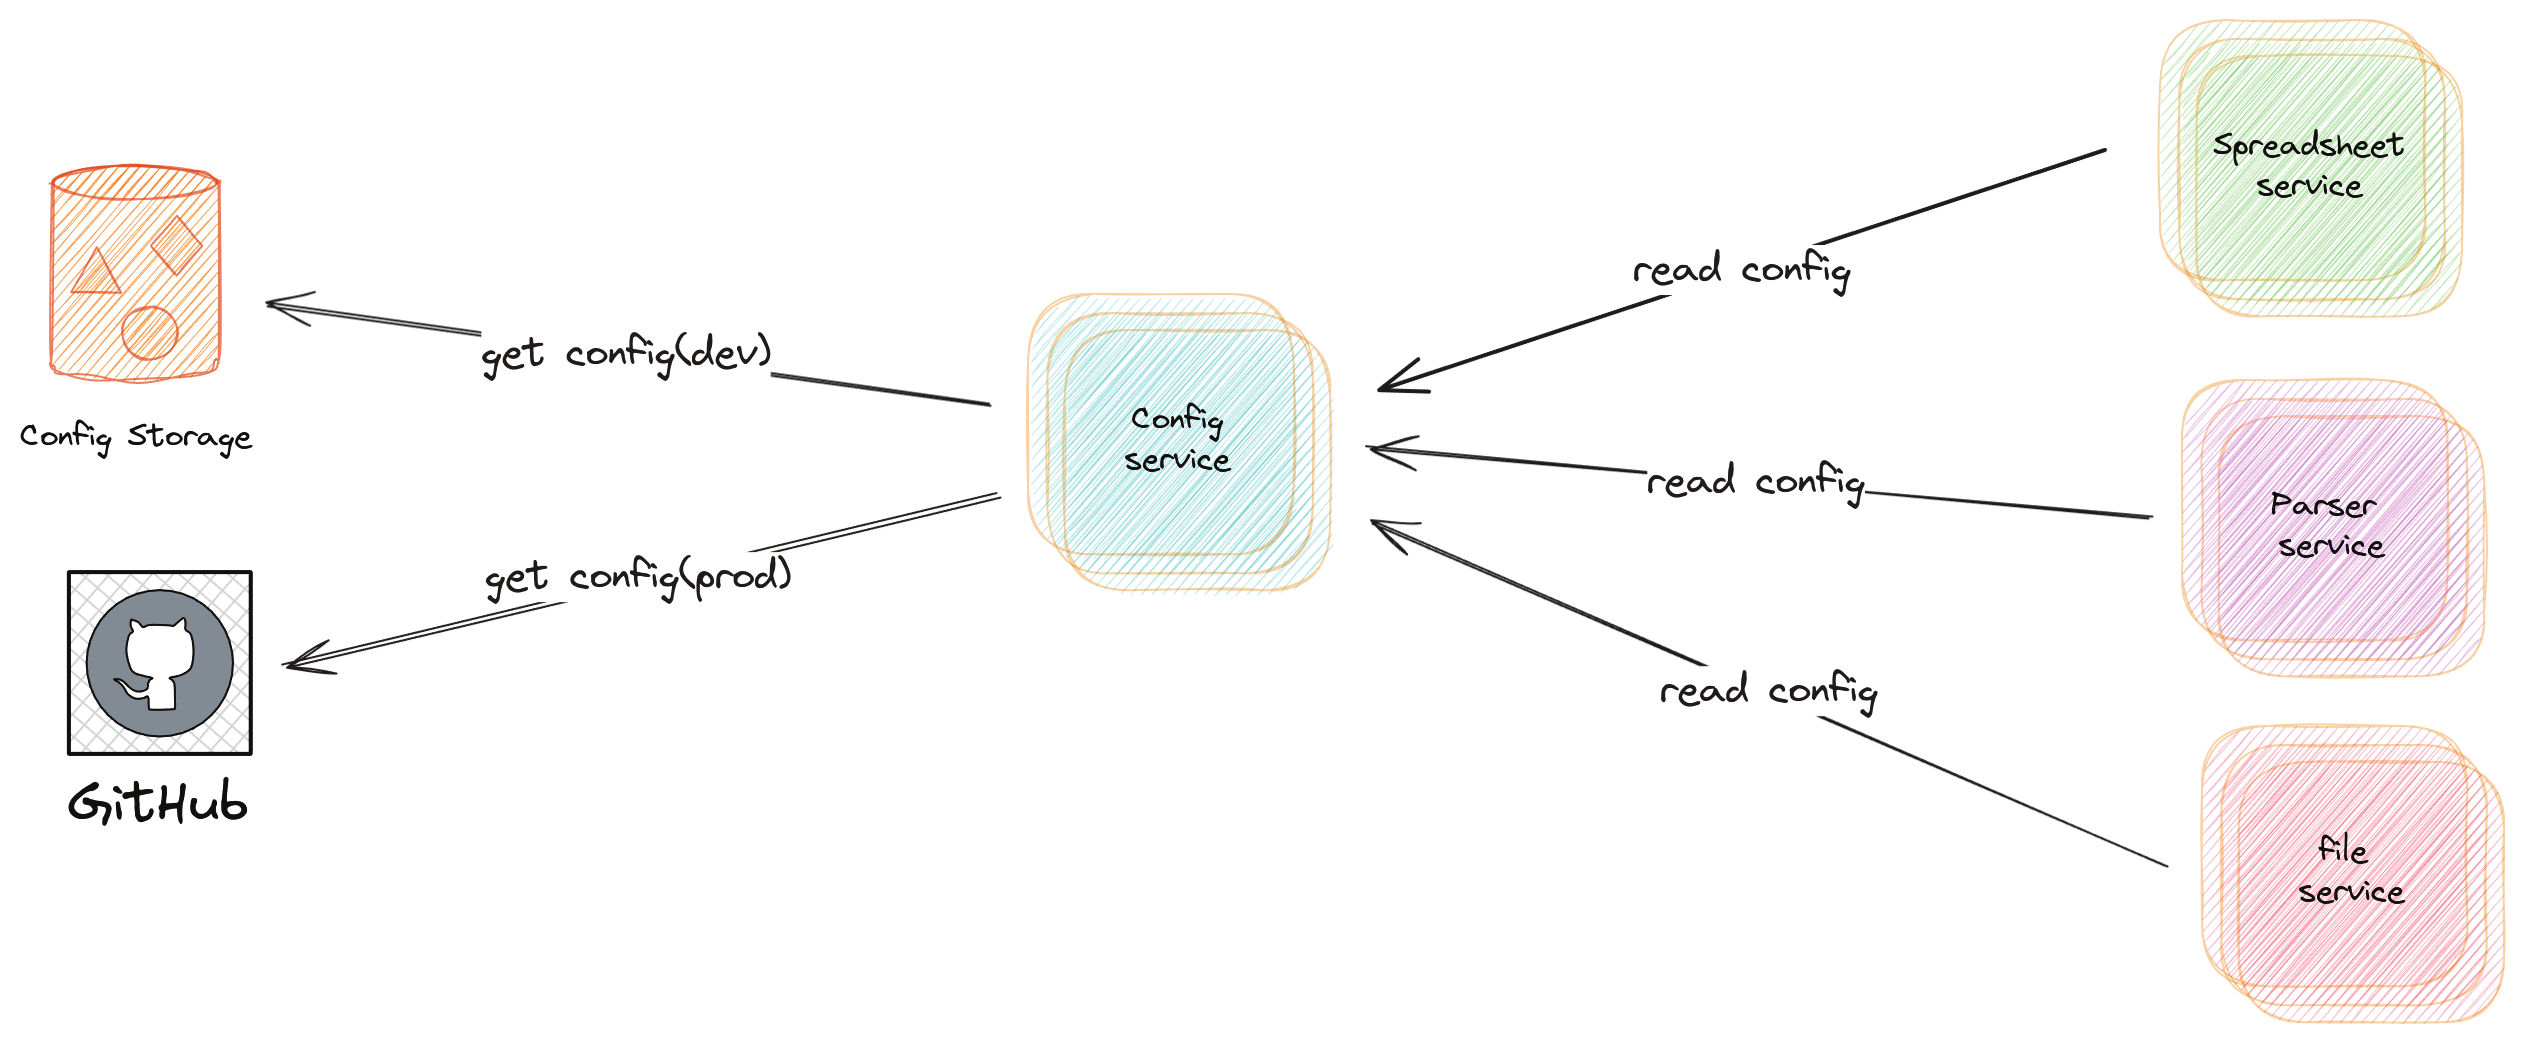
\includegraphics[width=0.7\textwidth]{Dissertation/images/cfg_project}
    \caption{Config Service}
    \label{fig:cfg_prj}
\end{figure}

\subsection{Механизмы обеспечения безопасности конфигурационных данных}

Spring Cloud Config предоставляет комплексный набор механизмов для защиты конфиденциальной информации. Аутентификация и авторизация доступа к конфигурационным данным реализуется через интеграцию с провайдерами идентификации, поддерживающими протокол OAuth 2.0. Платформа обеспечивает нативную интеграцию с такими решениями, как Auth0, Okta и Keycloak, что позволяет реализовать гибкие схемы управления доступом.

Защита конфиденциальных данных, включая учетные записи и API-ключи, осуществляется посредством криптографического шифрования на уровне хранения. Использование Java Cryptography Extension (JCE) и интеграция с внешними системами управления секретами, такими как HashiCorp Vault, обеспечивает многоуровневую защиту критически важной информации. Применение TLS-шифрования для всех коммуникаций между клиентами и сервером конфигурации гарантирует защиту от перехвата и модификации данных в процессе передачи.

\subsection{Стратегии обеспечения отказоустойчивости}

Достижение высокой доступности сервиса конфигурации требует применения комплекса архитектурных решений. Развертывание множественных экземпляров Spring Cloud Config Server в кластерной конфигурации с использованием балансировщика нагрузки обеспечивает устойчивость к отказам отдельных узлов. Репликация конфигурационных репозиториев с автоматическим переключением на резервные хранилища минимизирует риски потери доступа к критически важным данным.

Особое значение приобретает механизм локального кеширования конфигураций на стороне клиентских приложений, что позволяет поддерживать работоспособность системы даже в условиях временной недоступности центрального сервера конфигурации. Данный подход обеспечивает graceful degradation функциональности без полной потери работоспособности.

\subsection{Интеграция с системами контроля версий}

Использование Git в качестве бэкенда для хранения конфигураций предоставляет возможности для управления изменениями, аудита и восстановления предыдущих состояний. Spring Cloud Config Server поддерживает работу как с удаленными, так и с локальными Git-репозиториями, обеспечивая гибкость в выборе стратегии хранения.

Базовая конфигурация Config Server с Git backend представлена следующим образом:

\begin{lstlisting}

  cloud:
    config:
      server:
        git:
          uri: https://github.com/company/microservices-config.git
          clone-on-start: true
          default-label: main
          timeout: 10
          force-pull: true
          delete-untracked-branches: true
          refresh-rate: 60
        health:
          repositories:
            config:
              label: main
              name: user-service
              profiles: development,production
management:
  endpoints:
    web:
      exposure:
        include: health,info,refresh,configprops
\end{lstlisting}

Реализация поддерживает использование параметризованных URL-адресов репозиториев с подстановкой значений для идентификаторов приложений и профилей, что позволяет реализовать политику изоляции конфигураций на уровне отдельных микросервисов. Данный подход обеспечивает гранулярный контроль доступа и упрощает управление правами в многокомандной среде разработки.

Пример конфигурации с параметризованными репозиториями:

\begin{lstlisting}
spring:
  cloud:
    config:
      server:
        git:
          uri: https://github.com/company/config-{application}.git
          repos:
            user-service:
              pattern: user-service*
              uri: https://github.com/company/user-service-config.git
              username: ${GIT_USERNAME}
              password: ${GIT_PASSWORD}
              search-paths: configs/{profile}
            order-service:
              pattern: order-service*,payment-service*
              uri: https://github.com/company/business-config.git
              clone-on-start: true
              search-paths:
                - order-service/{profile}
                - payment-service/{profile}
            default:
              pattern: "*"
              uri: https://github.com/company/common-config.git
              default-label: main
              search-paths: common,shared/{application}
\end{lstlisting}

Для обеспечения безопасности и аутентификации реализована поддержка различных методов авторизации:
\begin{lstlisting}
@Configuration
@EnableConfigServer
public class ConfigServerConfig {

    @Bean
    @ConfigurationProperties("spring.cloud.config.server.git")
    public MultipleJGitEnvironmentRepository gitEnvironmentRepository() {
        MultipleJGitEnvironmentRepository repository =
            new MultipleJGitEnvironmentRepository();

        // Настройка SSH ключей
        if (StringUtils.hasText(sshPrivateKey)) {
            repository.setHostKeyAlgorithm("ssh-rsa");
            repository.setPrivateKey(sshPrivateKey);
            repository.setKnownHostsFile(knownHostsFile);
            repository.setStrictHostKeyChecking(false);
        }

        return repository;
    }

    @Bean
    public EnvironmentEncryptorEnvironmentRepository environmentEncryptor(
            EnvironmentRepository delegate) {
        return new EnvironmentEncryptorEnvironmentRepository(delegate);
    }
}
\end{lstlisting}

\subsection{Перспективы развития технологии}

Дальнейшее развитие архитектуры централизованного управления конфигурациями предполагает углубление интеграции с современными инструментами оркестрации. Потенциальный переход на распределенные системы хранения конфигураций, такие как etcd, может обеспечить улучшенные характеристики масштабируемости и согласованности в условиях географически распределенных развертываний. Автоматизация процессов валидации и тестирования конфигураций с использованием методов формальной верификации представляет перспективное направление для повышения надежности системы.
